%------------------------------------------------------------------------------
\section{Modelo de Información: Proceso de gestión de proyectos}


\subsection{Descripción General}
En la figura \ref{fig:MOD01} se muestra la estructura de información que se manejara para el sistema de gestión de proyectos

\begin{figure}[htb]
\centering
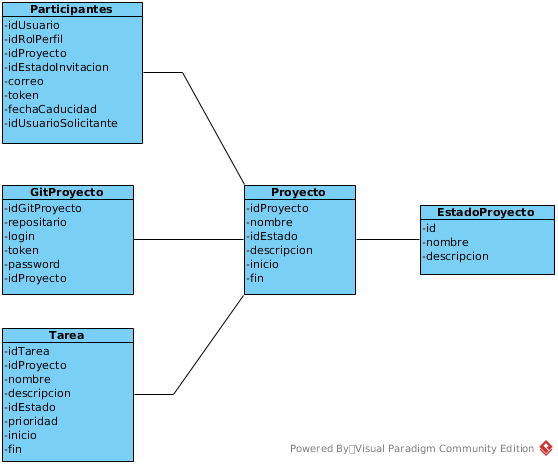
\includegraphics[width=0.8\textwidth]{./images/Modelo_Gestion_Proyectos.png}
\caption{Descripción general: Gestión de proyectos.} \label{fig:MOD01}
\end{figure}

\newpage

\subsection{Proyecto}

\begin{itemize}
	\item \textbf{Nombre} Denominación que se le da al proyecto. Es una palabra corta y este dato es requerido (no se puede omitir). Este atributo debe contener a lo mas 50 caracteres.
	\item \textbf{Descripción} Descripción de lo que trata el proyecto. Es una frase o enunciado, este dato es opcional. Este atributo debe contener a lo mas 100 caracteres.
	\item \textbf{Fecha de inicio} Fecha con la cual se indica el inicio del proyecto. Es una fecha dada en el formato dd/MMM/yyyy, este es un dato requerido (no se puede omitir).
	\item \textbf{Fecha de término} Fecha con la cual se indica el término del proyecto. Es una fecha dada en el formato dd/MMM/yyyy, este es un dato requerido (no se puede omitir).
	\item \textbf{Estado} Estado en que se encuentra el proyecto. Es dado por las diferentes situaciones en el proyecto.
\end{itemize}

\subsection{Repositorio Git}

\begin{itemize}
	\item \textbf{Repositorio} Es la URI del proyecto git que se quiere asociar con el proyecto. Es una URI la cual se obtiene desde tu repositorio git.
	\item \textbf{Token} Es una cadena la cual permite identificar al repositorio git. Es una cadena de caracteres que permite identificar si es posible conectarse al repositorio a traves de la aplicación
	\item \textbf{•}
\end{itemize}

\subsection{Participante}
\begin{itemize}
	\item \textbf{Proyecto} Es el proyecto del cual el particpante es miembro.
	\item \textbf{Estado Invitacion} Es el estado en el que se encuentra la invitacion del participante. Es dado a traves de las diferentes fases en las que se realiza el ciclo de vida de una invitación
\end{itemize}